	\section {Virtualization concepts}\label{sec:concetposVirtualizacion}	
	
	This section presents some of the terms used in virtualization. 
	It begins with a general description of the concept of \textit{virtualization}, followed by the categories called \textit{elements} and \textit{virtualization techniques}.
	
	\subsection{Virtualization}
	
	%Virtualization is the combination of different technologies, which offer advantages to organizations. 
	Virtualization is a combination of technologies that can help with the management of large volumes of data, with rapid scalability of infrastructure and with effectively utilizing a shared set of massive computing capabilities. According to \textit{Kusnetzky} \cite{Kusnetzky2011}, virtualization makes it possible to make an abstraction of applications and underlying hardware components in a logical or virtual view of these resources \cite{AbdElRahem2016}. This virtual view can sometimes be noticeably different from the physical view of computing resources, such as processing power, memory, storage capacity or even network bandwidth \cite{Stallings2015}. In addition to the above, \textit{Silberschatz} \cite{Silberschatz2014} notes that virtualization is technology that allows operating systems to run as applications within other operating systems.
	
	%La virtualización también incluye el término \textit{emulación}, el cual es ampliamente conocido y hace referencia al hecho de tener diferencias entre la arquitectura base y la proyectada en el proceso de virtualización.
	
	%JNM  you could expand this a bit saying how a virtual machine could be the same architecture,  a variant of the same architecture with strategic modifications to make virtualization easier or a completely different architecture. 
	
	%LESR - old - Before JNM
	%Virtualization also includes the term \textit{emulation}, which is widely known and refers to the fact that there are differences between the base architecture and the architecture projected in the virtualization process.
	
	%LESR - new
	Virtualization also includes the term \textit{emulation}, which is widely known and refers to the fact that there are differences between the base architecture and the architecture projected in the virtualization process. That is, a virtual machine could have the same host architecture, a variant of the same architecture with strategic modifications to make virtualization easier or a completely different architecture.
	
	%Entre los objetivos de la virtualización se tiene: aumento de los niveles de rendimiento computacional, favorecer la escalabilidad y disponibilidad de sus soluciones tecnológicas de manera eficiente y eficaz, además de propender por unificar y usar de forma fácil las estructuras de administración y seguridad de la infraestructura computacional existente \cite{Kusnetzky2011}, \cite{Hui2014}. 
	
	%JNM not sure what you mean hear by "increasing the levels of computational performance"? do you mean increasing performance? or do you mean having different levels of abstraction?
	
	%LESR - new
	Some virtualization goals include increasing the levels of use of computational resources, favoring scalability and availability unifying and helping to use the administration and security structures of the existing computational infrastructure \cite{Kusnetzky2011}, \cite{Hui2014}.
	
	%JNM this paragraph seems quite clear to me  - good... the one above referencing Kusnetzky2011 and Hui2014 seemed less clear
	
	%LESR - new
	Through virtualization, it is possible to create a logical view that combines computational resources that can represent one or more operating environments. This means, for example, that many physical computers look like a single great resource (aggregation of resources) or, on the contrary, that a single machine is considered as several instances of itself (division of resources) \cite{Silberschatz2014}. Virtualization can take place using methodologies, such as partition or aggregation of hardware and software, partial or complete machine simulation, emulation and time sharing among others \cite{Chiueh2005, Hoopes2009}. The separation of resources is one of the most common ways of using virtualization. In this case, it is possible to add the virtualization layer on top of real machine. This virtualization layer allows multiple virtualized environments to run simultaneously on the same real computer, either with the same architecture as the underlying system, with a variant of the same architecture including strategic modifications to facilitate virtualization, or with a completely different architecture for each particular need.
 

	
	%JNM Figure 1 and 3 were the same in the paper copy I have? Remove one?
	%\begin{figure}[!hbtp]
	%	\centering
	%	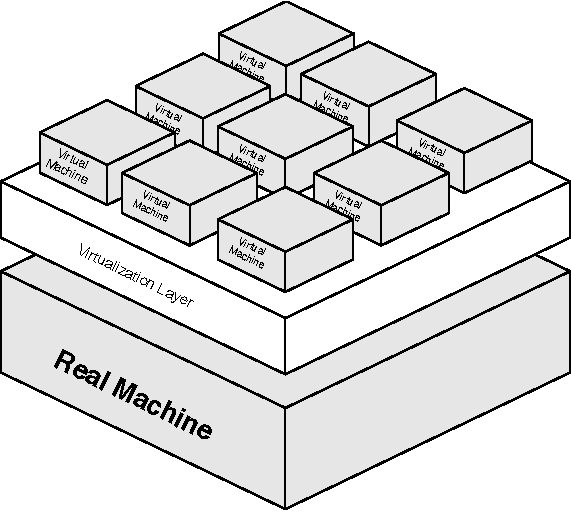
\includegraphics[width=7cm]{images/divisionRecursosFisicosConV12N.pdf}
	%	\vspace{-0.2cm}
	%	\caption{Division of resources through virtualization}
	%	\label{fig:divisionDeRecursosConVirtualizacion}
	%\end{figure}
	
	%JNM - this is also a place you could connect to the idea of virtualizing the same architecture, a variant of the same with strategic changes to make it easier to virtualize or completely different
	
	%LESR See above (Final part of the paragraph).
	
	Unfortunately, the x86 computer architecture, despite being one of the most widely adopted computer architecture in the world can not be virtualized completely\cite{Adams}. In this architecture, when executing instructions in non-privileged mode, some of them can fail silently instead of causing a trap and thus can not provide their respective treatment. 
	This situation can be solved through mechanisms and  virtualization approaches that act on different levels of abstraction. The abstraction levels where the virtualization takes place are the following: instruction set level, hardware abstraction level (HAL), operating system level (OS Level using system call interface), user-level library interface level and the application level \cite{Chiueh2005}. The virtualization concepts are grouped into the categories \textit{elements} and \textit{virtualization techniques}, which are described below.
	
	\subsection{Elements of virtualization}
	
	The elements \textit {real machine}, \textit {virtual machine} and \textit {virtual machine monitor}, are fundamental for understanding the virtualization technologies.
	These elements are described as follows.
	
	\subsubsection{Real machine}
	
	The term \textit{real machine} refers to the physical elements of the technological infrastructure that make up a computer; be it a personal computer, a workstation or a server. 
	Other references to this term are \textit {hardware}, \textit {physical hardware}, and \textit{bare-metal}. 
	In the commercial computer field, it is common to refer to the real machine concept using the word \textit{host} \cite{VMware2008}.
	
	\subsubsection{Virtual machine}
	
	The concept of \textit{virtual machine} (VM) is not new and was formalized in \textit{Goldberg}'s thesis in 1973 \cite {Goldberg1973} and published in various academic works in 1974 \cite{Popek1974}, \cite{Goldberg1974}. In these studies, virtual machine is defined as an efficient and isolated duplicate of the real machine, see Figure \ref{fig:TheVirtualMachineMonitor_Popek1974}. In later works, the term virtual machine has been extended to include other kinds of virtualization including applications at user level such as libraries, system calls, interfaces/services, system configurations, processes and state files \cite{Chiueh2005}. Another way of showing this concept is to relate to a software layer, which is put between the hardware or software resources and the applications \cite{Solis2014}. It is also very common in the commercial computing field to refer to the concept of VM using the word \textit{guest} \cite{VMware2008}. Finally, a virtual machine also is considered as an abstraction of computing resources presented as a service to allow them to operate simultaneously on the same real machine infrastructure \cite{Pek2013}.

%    \begin{center}
%		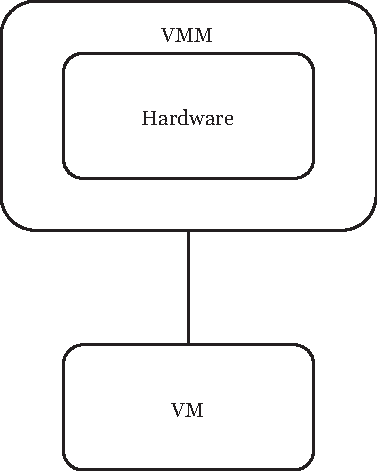
\includegraphics[width=3cm]{images/TheVirtualMachineMonitor_Popek1974.pdf}
%		\vspace{-0.2cm}
%        \captionof{figure}{Overview of virtual machine (VM) and virtual machine monitor (VMM)\footnotemark[2]{}.}
%        \label{fig:TheVirtualMachineMonitor_Popek1974}
%    \end{center}

	\begin{figure}[H]
		\centering
		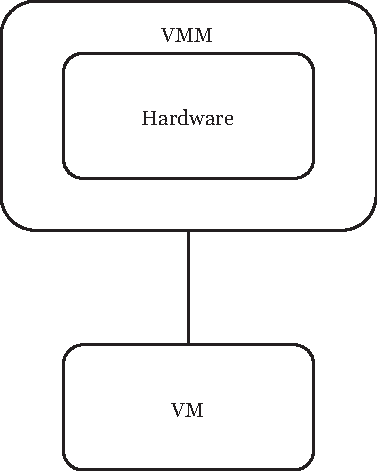
\includegraphics[width=3cm]{images/TheVirtualMachineMonitor_Popek1974.pdf}
		\vspace{0.2mm}
		\caption{Overview of virtual machine (VM) and virtual machine monitor (VMM) \cite{Popek1974}. }
		\label{fig:TheVirtualMachineMonitor_Popek1974}
	\end{figure}
	
	\subsubsection{Virtual machine monitor}
	
	The term \textit{virtual machine monitor} (VMM), was established by \textit{Popek} and \textit{Goldger} \cite{Popek1974}, in which they have defined the conceptual foundation of VMM as a piece of software that has three essential characteristics: \textbf{Equivalence}: To provide an execution environment for programs. This environment is identical to the original machine. \textbf{Performance}: Programs that run in this environment show, in the worst case, only minor decreases in speed. \textbf{Resource Control}: The VMM is in complete control of the system resources. The definition of a VMM is related to a software layer that provides support infrastructure using the resources of a lower level (usually \textit{hardware}), to create multiple VMs that are independent and isolated from each other \cite{Chiueh2005}, \cite{Cafaro2011}. Similarly, \textit{William Stallings} \cite{Stallings2015} determines that a VMM, is software that acts as an intermediary between the real machine and the VMs. 
	This software is commonly called \textit{Hypervisor} and it allows many VMs to coexist safely in the same hardware. The number of VMs that exist in a single computer determines the index of consolidation. In the particular case of Figure \ref{fig:VMM}, 9 to 1 is expressed as (9:1). The higher the consolidation index, the better the ROI and the less the TCO of the real machine used. Some of the functions and responsibilities of hypervisors are; emulation, isolation, resource allocation, and encapsulation \cite{Hoopes2009}.

%    \begin{center}
%		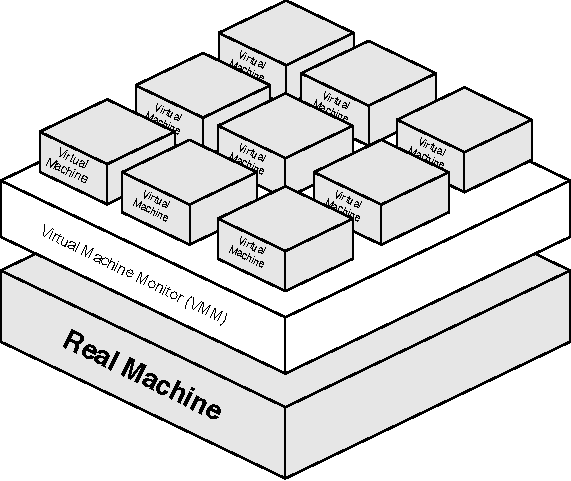
\includegraphics[width=6cm]{images/VMM.pdf}
%       %\vspace{1mm}
%        %\parbox[c]{8.3cm}{\footnotesize{Fig.1.~}  Example for inserting a one-column wide figure. }%
%        \vspace*{.2mm}
%        \captionof{figure}{Virtual Machine Monitor (VMM) or Hypervisor}
%        \label{fig:VMM}
%    \end{center}

    \begin{figure}[H]
        \centering
        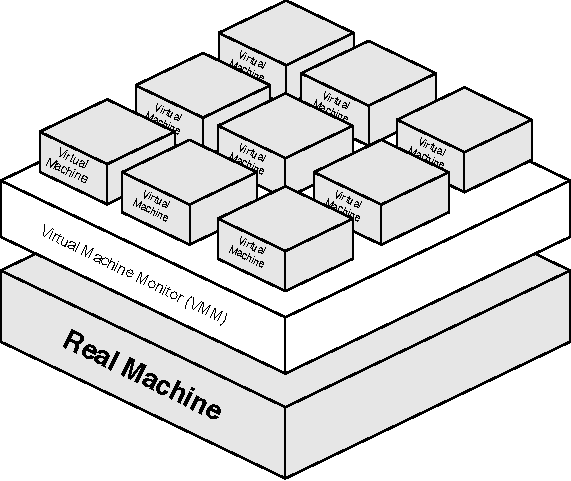
\includegraphics[width=6cm]{images/VMM.pdf}
        \vspace{0.2mm}
        \caption{Virtual Machine Monitor (VMM) or Hypervisor}
        \label{fig:VMM}
    \end{figure}

	\subsection{Virtualization techniques}
	
	The virtualization techniques called \textit{based on hypervisor} and \textit {based on containers} are described below. 
	These techniques are popular because they make it possible to consolidate hardware components easily.
	
	\subsubsection{Hypervisor-based virtualization technique}
	
	This virtualization technique consists of using the hypervisor as a central element, which takes in two different forms. The first one, is to locate the hypervisor directly onto the hardware. 
	This technique is also known as virtualization \textit{bare-metal} or \textit{native}, and the hypervisor is considered to be \textit{Type-1} (see Figure \ref{fig:Bare-metalHypervisor}). 
	The installation of this type of hypervisor does not need the presence of an underlying operating system. The second  form is to install the hypervisor on an existing operating system. 
	This technique is also known as virtualization \textit{hosted} or \textit{host-based}, and the hypervisor is considered to be \textit{Type-2} (see Figure \ref{fig:host-basedHypervisor}). 
	The main feature of Hypervisor-based virtualization is to create a fully operational virtual machine. This virtual machine can run independently and possibly on top of a different \textit{guest} operating systems, as long as they are compatible with delivered virtual architecture.

	\begin{figure}[H]
		\centering
		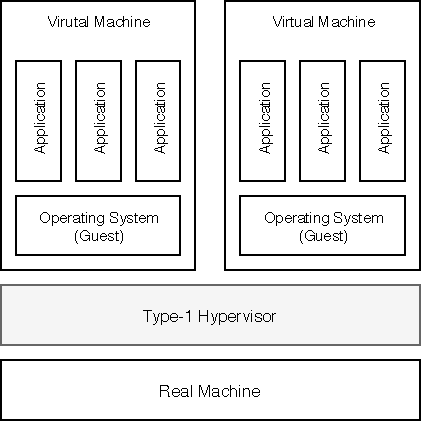
\includegraphics[width=6cm]{images/bare-metalHypervisor.pdf}
		\vspace{-0.2cm}
		\caption{Bare-metal Hypervisor}
		\label{fig:Bare-metalHypervisor}
	\end{figure}
	
	\begin{figure}[H]
		\centering
		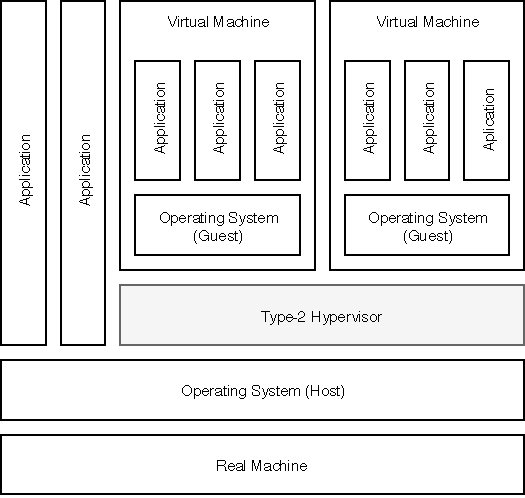
\includegraphics[width=6cm]{images/hosted-BasedHypervisor.pdf}
		\vspace{-0.2cm}
		\caption{Host-based hypervisor}
		\label{fig:host-basedHypervisor}
	\end{figure}
	
	\subsubsection {Container-based virtualization technique}
	
	This virtualization technique is based on a pre-existing operating system and consists of the generation of virtual execution environments for processes. 
	These execution environments are commonly called \textit{Containers} (see figure \ref{fig:container-baseVirtualization}). This virtualization technique requires fundamental parts of the OS to generate the virtual operating environments for the processes \cite{Kon2017}.
	Unlike hypervisor-based virtualization, which is required to generate VMs with whole operating systems,\cite{Kon2017}. 
	
	%This absence of OS supposes a lower computational load necessary to generate the virtual environment and in the same way, assumes that said environment is subject to the type of underlying operating system. 
	
	Avoiding the need for a separate OS in each container lowers the computational resources needed to support each container, but reduces flexibility because each container must have the same OS type and version. 

	\begin{figure}[H]
		\centering
		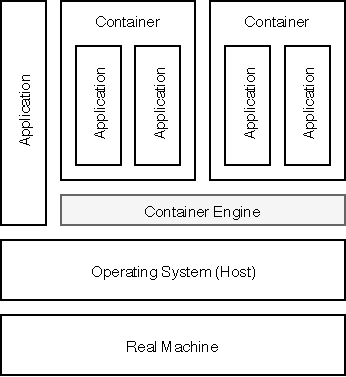
\includegraphics[width=6cm]{images/container-BasedVirtualization.pdf}
		\vspace{-0.2cm}
		\caption{Container-based virtualization}
		\label{fig:container-baseVirtualization}
	\end{figure}
	